\documentclass{beamer}

\usepackage{kotex}
\usepackage{graphicx}
\usepackage{minted}
\usepackage[export]{adjustbox}

\vfuzz=30pt

%%%%%%%%%%%%%%%%%%%%%
%  Beamer Settings  %
%%%%%%%%%%%%%%%%%%%%%
\usetheme[numbering=fraction]{metropolis}
\usecolortheme{rose}
\useoutertheme[subsection=false]{miniframes}

\setbeamertemplate{itemize item}[square]
\setbeamertemplate{itemize subitem}[triangle]
\setbeamertemplate{itemize subsubitem}[circle]

%%%%%%%%%%%%%%%%%%%
%  Font Settings  %
%%%%%%%%%%%%%%%%%%%
\usepackage[factor=500]{microtype}

\usepackage[mathrm=sym]{unicode-math}

\setmainfont{TeXGyrePagellaX}
\setsansfont{Roboto}[
  BoldFont = *-Medium,
  BoldItalicFont = *-MediumItalic
]
\setmonofont{Inconsolata}

\setmainhangulfont{NanumMyeongjo}
\setsanshangulfont{NanumGothic}[AutoFakeSlant=0.18]

\setmathfont{Fira Math}
\setmathfont{Fira Sans Medium}[range=bfsfup]
\setmathfont{Fira Sans Medium Italic}[range=bfsfit]
\setmathfont{STIX Two Math}[range=cal]

%%%%%%%%%%%%%%%%%%%%%
%  Minted Settings  %
%%%%%%%%%%%%%%%%%%%%%
\renewcommand\theFancyVerbLine{\textsf{\tiny\arabic{FancyVerbLine}}}

\newminted{latex}{
  escapeinside=||,
  autogobble,
  linenos,
  breaklines,
  numbersep=5pt,
  frame=single,
  fontsize=\scriptsize}
\newmintinline[ltxverb]{latex}{}

%%%%%%%%%%%%%%%%%%%%%%%
%  Document Settings  %
%%%%%%%%%%%%%%%%%%%%%%%

\title{%
  {\large memoir와 expl3로 해보는 Book Design}\\
  Page Style
}

\author{이재호}
\institute{memoir 스터디 그룹}
\date{\today}

%%%%%%%%%%%%%%
%  Document  %
%%%%%%%%%%%%%%
\begin{document}

\maketitle

\section{Make Page Style}

\begin{frame}[fragile]{\texttt{\textbackslash make[even|odd][head|foot]}}
  \begin{columns}
    \begin{column}{0.6\textwidth}
      \begin{latexcode}
        \makepagestyle{demo}
        \makeevenhead{demo}{ehl}{ehc}{ehr}
        \makeoddhead{demo}{ohl}{ohc}{ohr}
        \makeevenfoot{demo}{efl}{efc}{efr}
        \makeoddfoot{demo}{ofl}{ofc}{ofr}
      \end{latexcode}
    \end{column}

    \begin{column}{0.4\textwidth}
      \begin{overprint}
        \onslide<1>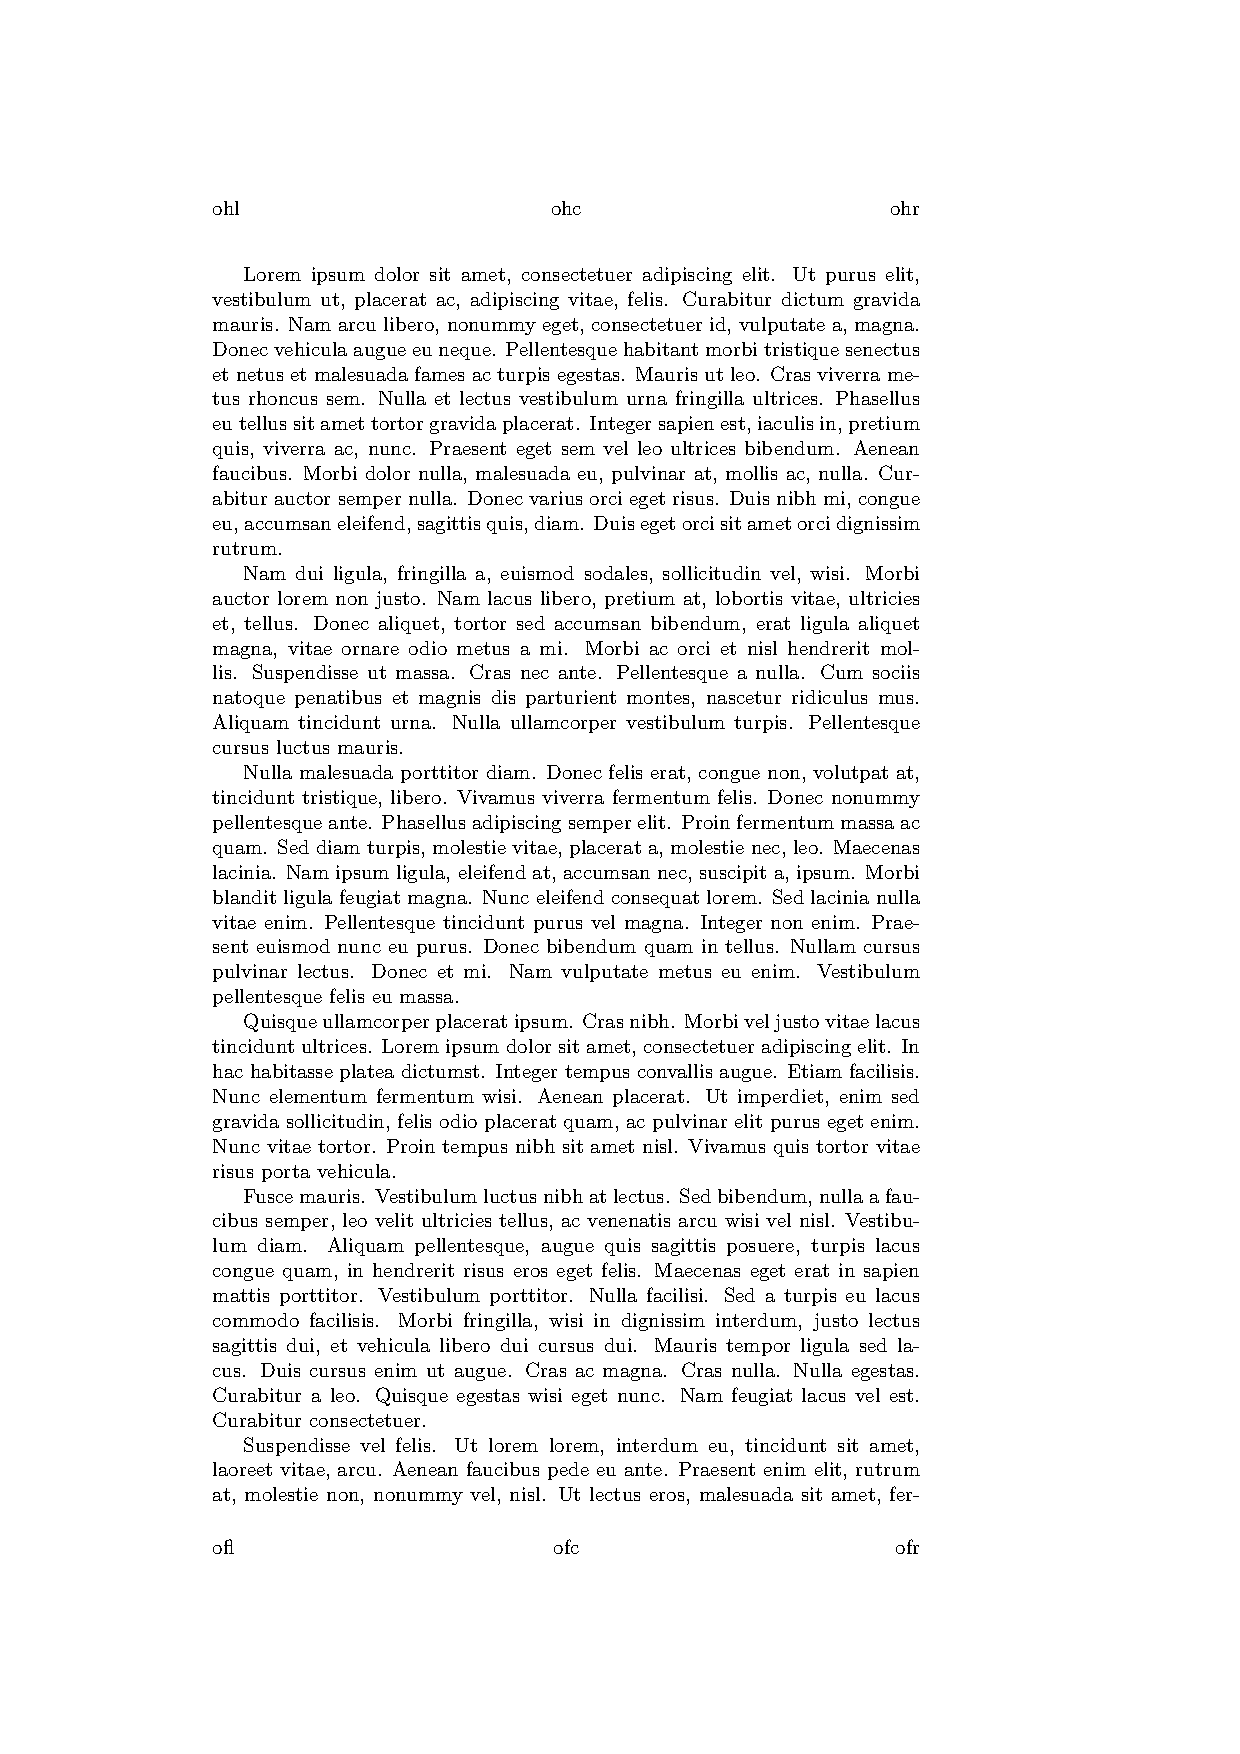
\includegraphics[frame,width=\linewidth]{demo-hf-1}
        \onslide<2>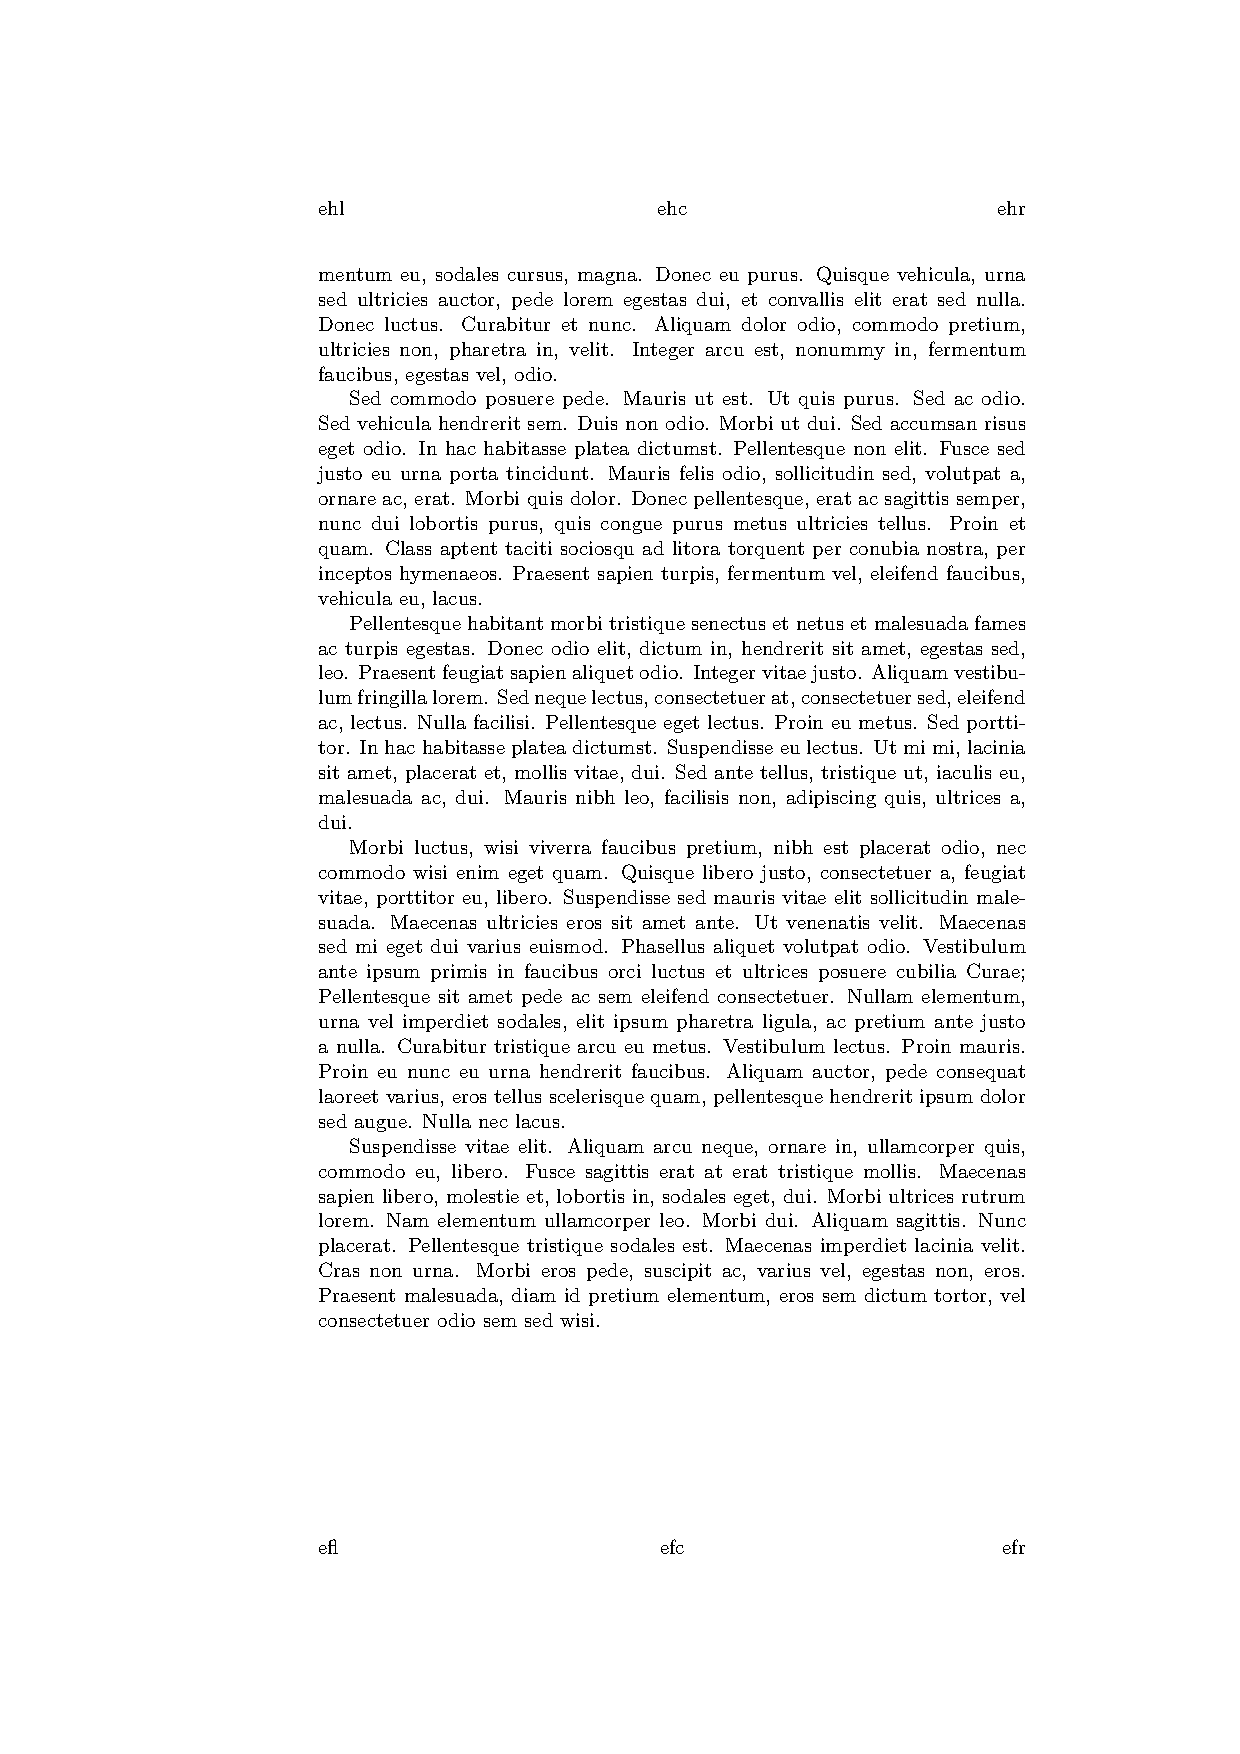
\includegraphics[frame,width=\linewidth]{demo-hf-2}
      \end{overprint}
    \end{column}
  \end{columns}
\end{frame}

\end{document}
